\documentclass{beamer}
\usepackage{hyperref}
\usepackage{CJK}
\usepackage{listings}
\usepackage{multicol}
\usepackage{tikz}
\usepackage{pdfpages}   
\usetikzlibrary{automata, positioning}

\graphicspath{ {./images/} }

\definecolor{mygreen}{rgb}{0,0.6,0}
\definecolor{mygray}{rgb}{0.5,0.5,0.5}
\definecolor{mymauve}{rgb}{0.58,0,0.82}
\definecolor{tiffanyblue}{rgb}{0.04, 0.73, 0.71}

\lstset{ 
  backgroundcolor=\color{white},   % choose the background color; you must add \usepackage{color} or \usepackage{xcolor}; should come as last argument
  basicstyle=\ttfamily\footnotesize,% the size of the fonts that are used for the code
  breakatwhitespace=false,         % sets if automatic breaks should only happen at whitespace
  breaklines=true,                 % sets automatic line breaking
  captionpos=b,                    % sets the caption-position to bottom
  commentstyle=\color{mygreen},    % comment style
  deletekeywords={...},            % if you want to delete keywords from the given language
  escapeinside={\%*}{*)},          % if you want to add LaTeX within your code
  extendedchars=true,              % lets you use non-ASCII characters; for 8-bits encodings only, does not work with UTF-8
  frame=single,	                   % adds a frame around the code
  keepspaces=true,                 % keeps spaces in text, useful for keeping indentation of code (possibly needs columns=flexible)
  keywordstyle=\color{red},        % keyword style
  morekeywords={\*, ...},          % if you want to add more keywords to the set
  numbers=left,                    % where to put the line-numbers; possible values are (none, left, right)
  numbersep=5pt,                   % how far the line-numbers are from the code
  numberstyle=\tiny\color{mygray}, % the style that is used for the line-numbers
  rulecolor=\color{black},         % if not set, the frame-color may be changed on line-breaks within not-black text (e.g. comments (green here))
  showspaces=false,                % show spaces everywhere adding particular underscores; it overrides 'showstringspaces'
  showstringspaces=false,          % underline spaces within strings only
  showtabs=false,                  % show tabs within strings adding particular underscores
  stepnumber=1,                    % the step between two line-numbers. If it's 1, each line will be numbered
  stringstyle=\color{mymauve},     % string literal style
  tabsize=4,	                     % sets default tabsize to ˋ spaces
}

\setbeamercolor{block title}{use=structure,fg=white,bg=purple!75!black}
\setbeamercolor{block body}{use=structure,fg=black,bg=white!20!white}
\setbeamertemplate{blocks}[rounded][shadow=false]

\AtBeginSection[]{
  \begin{frame}
  \vfill
  \centering
  \begin{beamercolorbox}[sep=8pt,center,shadow=true,rounded=true]{title}
    \usebeamerfont{title}\insertsectionhead\par%
  \end{beamercolorbox}
  \vfill
  \end{frame}
}

\hypersetup{
    colorlinks = true,
    linkbordercolor = {white},
    linkcolor=blue
}

\begin{document}
\begin{CJK*}{UTF8}{bsmi}

    \title{Intro. to Secure Programming}
    \subtitle{Study Groups at NCYU}
    \author{Chih-Hsuan Yang(SCC)}
    \institute{\href{mailto:zxc25077667@pm.me}{zxc25077667@pm.me}}

    \begin{frame}
        \titlepage
    \end{frame}

    \begin{frame}{About me}
        \begin{itemize}
            \item 楊志璿
            \item NSYSU Information security club founder
            \item \href{https://github.com/25077667/Resume/blob/main/resume/resume.pdf}{Resume}
            \item Linux, Modern C++
        \end{itemize}
    \end{frame}

    \begin{frame}{A book}
        \href{https://dwheeler.com/secure-programs/}{Secure Programming}\\
        Not hard, no much pages.
    \end{frame}

    \begin{frame}{Outline}
        \tableofcontents
    \end{frame}

    \section{Background}
    \begin{frame}{Maslow’s pyramid of code review}
        \centering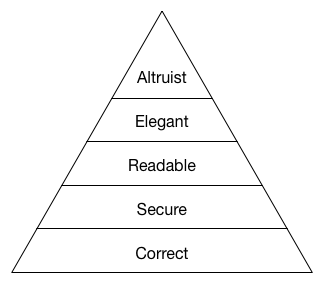
\includegraphics[height=.9\textheight]{Maslow.png}
    \end{frame}

    \begin{frame}{Maslow’s pyramid of code review}
        \begin{itemize}
            \item  Correct  : 做到預期的行為了嗎?能夠處理各式邊際狀況嗎?即便其他人修改程式碼後,主體的行為仍符合預期嗎?
            \item  \underline{Secure : 面對各式輸入條件或攻擊,程式仍可正確運作嗎?}
            \item  Readable : 程式碼易於理解和維護嗎?
            \item  Elegant  : 程式碼夠「美」嗎?可以簡潔又清晰地解決問題嗎?
            \item  Altruist : 除了滿足現有的狀況,軟體在日後能夠重用嗎?甚至能夠抽離一部分元件,給其他專案使用嗎?
        \end{itemize}
    \end{frame}

    \section{Programmer's qualities}

    \subsection{Arithmetic overflow}
    \begin{frame}{Arithmetic overflow}
        \centering
        \begin{tabular}{ |p{2cm}||p{1cm}|p{1cm}|p{1cm}|p{1cm}|p{1cm}|  }
            \hline
            \multicolumn{6}{|c|}{Data Model}                \\
            \hline
            Type      & LP32 & ILP32 & LP64 & ILP64 & LLP64 \\
            \hline
            char      & 8    & 8     & 8    & 8     & 8     \\
            short     & 16   & 16    & 16   & 16    & 16    \\
            int       & 16   & 32    & 32   & 64    & 32    \\
            long      & 32   & 32    & 64   & 64    & 32    \\
            long long & 64   & 64    & 64   & 64    & 64    \\
            pointer   & 32   & 32    & 64   & 64    & 64    \\
            \hline
        \end{tabular}
    \end{frame}

    \begin{frame}{Bits field}
        \centering
        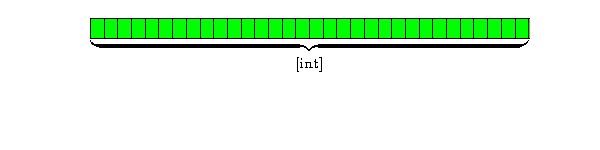
\includegraphics[width=\textwidth]{src/mem_layout/mem.pdf}
    \end{frame}

    \begin{frame}{2's complement}
        Eg:
        \begin{itemize}
            \item 0x1234ABCD
            \item 0x00BADBAD
            \item 0xFFFFFFFF
        \end{itemize}
    \end{frame}

    \begin{frame}{Integer overflow}
        2002 FreeBSD
        \lstinputlisting[language=C]{src/bsd.c}
        What if maxlen $<$ 0?\\
        Take maxlen as -1, try it!
    \end{frame}

    \begin{frame}{Integer overflow}
        2002 External data representation (XDR)
        \lstinputlisting[language=C]{src/malloc0.c}
        What if ele\_cnt = $10^{22}$, ele\_size = $10^{10}$ ?\\
        Try it!
    \end{frame}

    \begin{frame}{Binary search}
        \lstinputlisting[xleftmargin=1em, language=C, linerange={1-15}, firstnumber=1]{src/bs.c}
    \end{frame}

    \begin{frame}{Binary search}
        \lstinputlisting[xleftmargin=1em, language=C, linerange={17-31}, firstnumber=1]{src/bs.c}
    \end{frame}

    \begin{frame}{Binary search}
        \begin{itemize}
            \item 1946 idea
            \item 1960 mathematical analysis
            \item 1988 find bugs.
        \end{itemize}
        \begin{block}{Donald Knuth}
            \setbeamercolor{block title}{bg=red!30,fg=black}
            Although the basic idea of binary search is comparatively straightforward, the details can be surprisingly tricky.
        \end{block}
    \end{frame}

    \begin{frame}{Appendix here - Donald Knuth}
        \begin{itemize}
            \item \TeX
            \item The Art of Computer Programming (TAOCP)
        \end{itemize}
        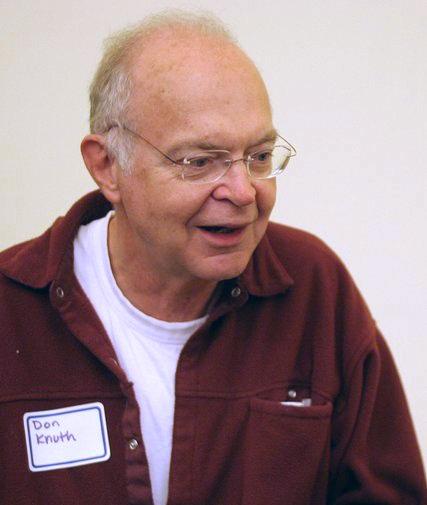
\includegraphics[height=.5\textheight]{Knuth.jpg}
    \end{frame}

    \subsection{ReDoS}
    \begin{frame}{ReDoS}
        \centering
        \begin{columns}
            \begin{column}{0.5\textwidth}
                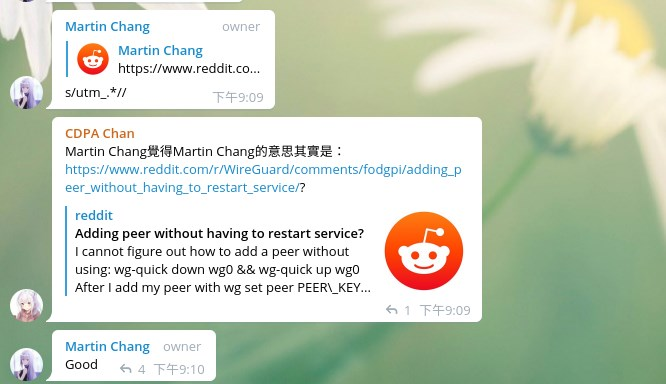
\includegraphics[width=1.1\textwidth]{redos1.jpg}
            \end{column}
            \begin{column}{0.5\textwidth}
                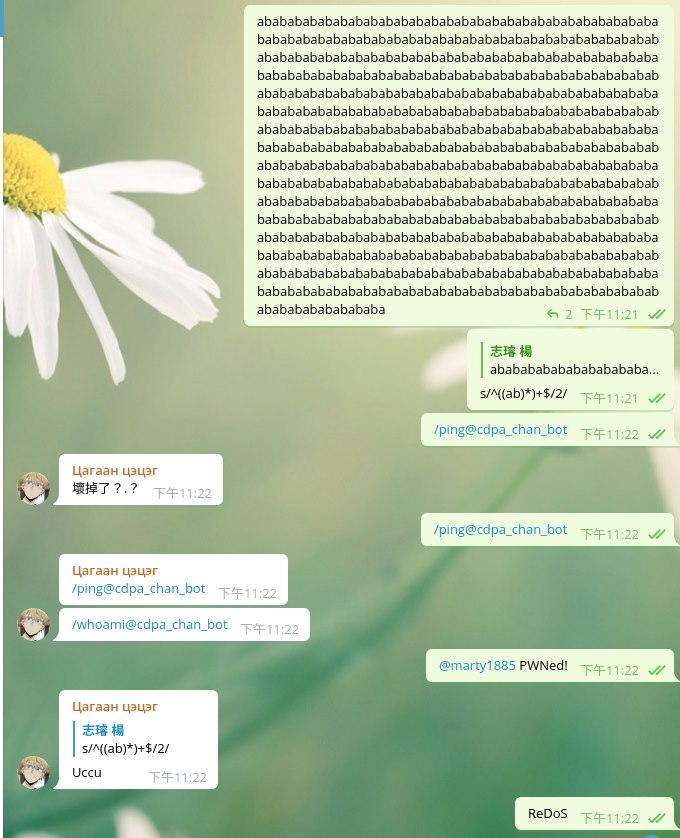
\includegraphics[width=1.1\textwidth]{redos2.jpg}
            \end{column}
        \end{columns}
    \end{frame}

    \begin{frame}{Regex}
        \begin{itemize}
            \item Regular expression
            \item Finite state machine
        \end{itemize}
        \centering
        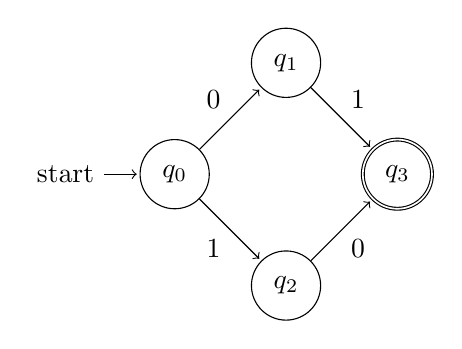
\begin{tikzpicture}[shorten >=1pt,node distance=2cm,on grid,auto]
            \node[state,initial] (q_0)   {$q_0$};
            \node[state] (q_1) [above right=of q_0] {$q_1$};
            \node[state] (q_2) [below right=of q_0] {$q_2$};
            \node[state,accepting](q_3) [below right=of q_1] {$q_3$};
            \path[->]
            (q_0) edge  node {0} (q_1)
            edge  node [swap] {1} (q_2)
            (q_1) edge  node  {1} (q_3)
            (q_2) edge  node [swap] {0} (q_3);
        \end{tikzpicture}
    \end{frame}

    \begin{frame}{Regex basic}
        \href{https://regex101.com/}{Regex 101}\\
        Let's try:\\
        \begin{itemize}
            \item A brown fox jumps over the lazy dog.
            \item Student ID.
            \item Binary search code.
            \item Email.
        \end{itemize}
    \end{frame}

    \begin{frame}{Halting problem}
        \^\ ((ab)*)+\$
        \newline
        \centering
        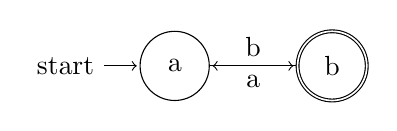
\begin{tikzpicture}[shorten >=1pt,node distance=2cm,on grid,auto]
            \node[state, initial] (q_0)   {a};
            \node[state, accepting] (q_1) [right=of q_0] {b};
            \path[->]
            (q_0) edge  node {b} (q_1)
            (q_1) edge  node {a} (q_0);
        \end{tikzpicture}
        \begin{block}{Input}
            ababababababababababababa
        \end{block}
    \end{frame}

    \begin{frame}{Halting problem}
        The engine will first try (abababababababababababab) but that
        fails because of that extra a. This causes catastrophic bracktracking,
        because our pattern (ab)*, in a show of good faith, will release
        one of it's captures (it will "backtrack") and let the outer
        pattern try again.
        \begin{itemize}
            \item (abababababababababababab) - Nope
            \item (ababababababababababab)(ab) - Nope
            \item (abababababababababab)(abab) - Nope
            \item (abababababababababab)(ab)(ab) - Nope
            \item (ababababababababab)(ababab) - Nope
            \item (ababababababababab)(abab)(ab) - Nope
            \item (ababababababababab)(ab)(abab) - Nope
            \item (ababababababababab)(ab)(ab)(ab) - Nope
            \item \dots
            \item (ab)(ab)(ab)(ab)(ab)(ab)(ab)(ab)(ab)(ab)(ab)(ab) - Nope
        \end{itemize}
    \end{frame}

    \begin{frame}{Halting problem}
        \begin{center}
            \LARGE
            $$dp[0] = 1$$
            $$dp[N]=\sum^{N}_{i=0}{dp[i] + dp[N-i]} $$
            $$\sim O(3^N) $$
        \end{center}
    \end{frame}

    \begin{frame}{ReDoS}
        So, please check what you did.\\
        User provides regex should have a timeout threshold.\\
        Don't believe the user inputs.
    \end{frame}

    \subsection{RAII}
    \begin{frame}{RAII}
        \begin{itemize}
            \item Resource Acquisition Is Initialization
            \item Bjarne Stroustrup
            \item Constructor, destructor
            \item Don't memorize.
        \end{itemize}
        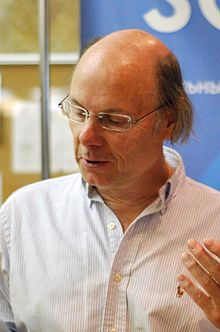
\includegraphics[height=.5\textheight]{Bjarne.jpg}
    \end{frame}

    \begin{frame}{RAII}
        lifetime
    \end{frame}

    \begin{frame}{RAII}
        objects, files, sockets, locks
    \end{frame}

    \begin{frame}{RAII}
        exceptions
    \end{frame}

    \section{Memory safe}
    \subsection{Buffer overflow}
    \begin{frame}{Buffer overflow}
        sample code.
    \end{frame}

    \begin{frame}{Buffer overflow}
        Try some code.\\
        strcpy, strncpy
    \end{frame}

    \begin{frame}{Buffer overflow}
        bof on stack
    \end{frame}

    \begin{frame}{Buffer overflow}
        canary
    \end{frame}

    \subsection{Memory leakage}
    \begin{frame}{Memory leakage}
        sample code
    \end{frame}

    \begin{frame}{Memory leakage}
        Try some codes.\\
        new, delete.
    \end{frame}

    \begin{frame}{Memory leakage}
        Garbage Collection
    \end{frame}

    \begin{frame}{Memory leakage}
        RAII
    \end{frame}

    \section{Call out to other routines}
    \subsection{Injections}
    \begin{frame}{SQL injection}
        not checking, string concatenation
    \end{frame}

    \begin{frame}{Command line injection}
        not checking, don't call commands directly.
    \end{frame}

    \section{Others}
    \subsection{Language features}
    \begin{frame}{Strong types, week types}
        Duck typing\\
        Philosophy
    \end{frame}

    \begin{frame}{Inheritance}
        Python
    \end{frame}

    \subsection{Authentication}
    \begin{frame}{Passwords}
        hash
    \end{frame}

    % \section{Labs}

\end{CJK*}
\end{document}